%% LyX 2.3.4 created this file.  For more info, see http://www.lyx.org/.
%% Do not edit unless you really know what you are doing.
\documentclass[oneside,english]{amsart}
\usepackage[T1]{fontenc}
\usepackage[latin9]{inputenc}
\usepackage{amsthm}
\usepackage{graphicx}
\usepackage{wasysym}
\usepackage[authoryear]{natbib}

\makeatletter
%%%%%%%%%%%%%%%%%%%%%%%%%%%%%% Textclass specific LaTeX commands.
\numberwithin{equation}{section}
\numberwithin{figure}{section}
\theoremstyle{plain}
\newtheorem{thm}{\protect\theoremname}
\theoremstyle{definition}
\newtheorem{example}[thm]{\protect\examplename}
\theoremstyle{plain}
\newtheorem{lem}[thm]{\protect\lemmaname}

\makeatother

\usepackage{babel}
\providecommand{\examplename}{Example}
\providecommand{\lemmaname}{Lemma}
\providecommand{\theoremname}{Theorem}

\begin{document}

\section{Ordinal alpha\label{sec:Ordinal alpha}}

Recall the congeneric model ((cite))

\[
X=\lambda Z+\Psi^{1/2}\epsilon
\]
Consider the scenario when we do not observe the $X_{i}$s directly,
but rather $X_{i}$s discretized into $m_{i}$ categories according
to

\begin{equation}
Y_{i}=k1[\tau_{i(k-1)}\leq X_{i}\leq\tau_{ik}],\label{eq:discretization model}
\end{equation}
where $-\infty=\tau_{i0}<\tau_{i1}<\ldots<\tau_{i(m_{i}+1)}=\infty$
are thresholds for each $i$ and $1[A]$ is the indicator function.
This is a common model for Likert scales with $m_{i}$ levels for
the $i$th item. If $X$ is multivariate normal, model (\ref{eq:discretization model})
is a congeneric \emph{multivariate ogive model} \citep{Swaminathan2016-rg}.
Under multivariate normality the correlation matrix $\Phi$ is point-indentified
from the distribution of $Y$, and is called the \emph{polychoric
correlation}. It can be estimated using maximum likelihood directly
or a two-step procedure \citep{Olsson1979-ti}. To make the model
identified, usual practice is assume $\Psi^{1/2}$ to be a correlation
matrix. 

\citet{Zumbo2007-ap} propose what I call the \emph{theoretical ordinal
alpha}

\begin{equation}
\alpha=\frac{k}{k-1}\left(1-\frac{k}{\mathbf{i}^{T}\Phi\mathbf{i}}\right)\label{eq:ordinal alpha}
\end{equation}
where $\Phi=\Cor X$ is polychoric correlation coefficient of $Y$.
Theoretical ordinal alpha is a standardized alpha, but it is based
on the latent correlation matrix between the unobserved $X$ instead
of the observed correlation matrix between the $Y$s. The population
values of the theoretical ordinal alpha and the standardized alpha
are not the same in general. \citet{Zumbo2007-ap}'s main argument
in favor of the ordinal alpha is ``coefficient alpha (and KR-20)
are correlation-based statistics and hence assume continuous data\textquoteright \textquoteright{}
\citep[p. 27]{Zumbo2007-ap}. \citet[p. 1060, "Misconcetion 1"]{Chalmers2018-fj}
persuasively argues against this idea, see also \citep{Raykov2019-yr}
and the section ((cite)) of this paper. The argument is reiterated
by \citep{Gadermann2012-jl}. However, \citet{Zumbo2019-lm} argue
the the benefit of sample ordinal alpha is that we are truly interested
in the reliability of $X$ as a predictor of $Y$ (in the parlance
of this paper). 

A related notion is the \emph{theoretical ordinal reliability, }the
analogue of the weighted reliability ((ref)) based on the polychoric
correlation coefficient. Its definition is 
\begin{equation}
\omega_{w}=\frac{w\lambda_{i}^{\star}}{w\lambda_{i}^{\star}+\sigma_{i}^{\star}}\label{eq:ordinal omega}
\end{equation}
were $\lambda_{i}^{\star}=\lambda_{i}/\sqrt{\lambda_{i}^{2}+\sigma_{i}^{2}}$
and $\sigma_{i}^{\star}=\sigma_{i}/\sqrt{\lambda_{i}^{2}+\sigma_{i}^{2}}$.

There several reasons to avoid the theoretical ordinal alpha. If your
goal is to estimate the congeneric reliability or the standardized
reliability, the theoretical ordinal alpha is inappropriate since
it does not equal the congeneric reliability, even under the parallel
model \citep[p. 1062, "Misconception 2"]{Chalmers2018-fj}, a point
conceded by \citet{Zumbo2019-lm}. But this is not the worst problem.
For even if you are interested in estimating the congeneric reliability
for the multivariate normal ogive model, you should avoid the theoretical
alpha.

Theoretical ordinal alpha is apparently not connected to any predictor
of $Z$ that depends on the data $Y$, only the correlation $\Cor^{2}(\sum_{i=1}^{k}w_{i}X_{i},Z)$.
This correlation is barely interesting though, since we do not observe
the latent $X_{i}$s. The theoretical alpha does not have the concrete
interpretation of the congeneric alpha mentioned in section 2, namely
``how good can I expected my prediction of $Z$ based on $X$ to
be?'', as $X$ is unknown and you cannot for your prediction. This
lack of knowledge about $X$ also makes correction for attenuation
impossible. Since $X$ is unknown, it is impossible to directly calculate
the correlation between a function of $X$ and a function of some
other quantity $X'$. Due to this, the correction for attuation formula
will not work. What you can calculate is the correlation between some
function of the observed variables $Y$ and a function of $X'$. 

Moreover, if you want the standardized reliability of the unobserved
$X$, the ordinal reliability is a better choice. For the conditions
required for standardized alpha to equal the standardized reliability
are still needed, i.e. the weighted $\tau$-equivalent model (). The
theoretical ordinal reliability can be estimated using e.g. $\mathtt{lavaan}$
without much added complexity. Using the same arguments as in the
previous section, the theoretical ordinal reliability with optimal
weights (corresponding to coefficient \emph{H}) or weights $w_{i}=\sigma_{i}$
(corresponding to the sigma reliabiltiy) should be prefered to the
standardized reliability too.

Finally, theoretical ordinal alpha only makes sense in relation to
the congeneric multivariate ogive model. But this model depends on
the fundamentally unverifiable assumption of multivariate normality
of $X$. The polychoric correlation coefficient is not robust against
normality in general \citep{Foldnes2019-yd}. 

\subsection{A concrete ordinal reliability}

The main argument of \citet{Zumbo2019-lm}'s rebuttal of \citep{Chalmers2018-fj}
is that the congeneric multivariate normal ogive model (\ref{eq:discretization model})
is a better approximation to reality than the congeneric model (ref).
So assume we believe in the discretized model and can be reasonably
sure that $X$ is multivariate normal. Then ordinal alpha would still
not be appropriate as it is theoretical and not concrete. However,
it is possible to create a class of reliability coefficients for the
multivariate normal discretized model.

Let $\widehat{X}_{i}$ be the mean of a standard normal distribution
truncated to $(\tau_{i(Y_{i}-1)},\tau_{iY_{i}}]$, or equivalently

\begin{equation}
\widehat{X}_{i}=-\frac{\phi(\tau_{iY_{i}})-\phi(\tau_{i(Y_{i}-1)})}{\Phi(\tau_{iY_{i}})-\Phi(\tau_{i(Y_{i}-1)})},\label{eq:Predictor of X}
\end{equation}
see \citep[Section 10.1]{Johnson1994-ag} for the formula for the
expectation of a truncated normal. Since $\widehat{X}_{i}$ is the
conditional expectation of $X_{i}$ given $Y_{i}$ it is the optimal
predictor of $X_{i}$ given $Y_{i}$ in the sense of minimizing the
mean squared error. A natural predictor of $Z$ given $Y$ is a linear
function of $\hat{X}_{i}$, i.e. $\sum_{i=1}^{k}w_{i}\hat{X}_{i}$
for some weights $w_{i}$, which gives rise to the analogue of the
weighted reliability (ref) in the context of the discretization model
(\ref{eq:discretization model}) when $X$ is multivariate normal
with standard normal marginals. Define the weighted ordinal reliability
as

\begin{equation}
\omega_{w}'=\Cor^{2}(\sum_{i=1}^{k}w_{i}\hat{X}_{i},Z).\label{eq:Weighted ordinal reliability}
\end{equation}
The following theorem shows how to calculate $\omega_{w}^{'}$ and
some of its properties.
\begin{thm}
\label{thm:omega-prime}Let $\hat{Z}=\sum_{i=1}^{k}w_{i}\hat{X}_{i}$
with $\hat{X}$ defined as in \ref{eq:Predictor of X} and $\Xi=\Cov\hat{X}$.
Assume $X$ is multivariate normal with standard normal marginals,
such that $\sqrt{\lambda_{i}^{2}+\sigma_{i}^{2}}=1$ for all $i$.
\begin{enumerate}
\item Let $v_{i}=$ be the Thurstone weights. Then $\sum_{i=1}^{k}w_{i}\hat{X}_{i}$
is the optimal predictor of $Z$, i.e. it minimizes the mean squared
error $\MSE(\hat{Z})$.
\item The weighted ordinal reliability is
\begin{eqnarray}
\omega_{w}' & = & \frac{(w^{T}\Xi v)^{2}}{w^{T}\Xi w}\label{eq:Omega prime}\\
 & = & 1-\MSE(v_{0}\hat{Z})\nonumber 
\end{eqnarray}
where $v_{i}=\lambda_{i}/[\sigma_{i}^{2}(1+k\overline{\lambda^{2}\sigma^{-2}})],\:i=1,\ldots,k$
are the Thurstone weights for $X$ and $v_{0}=w^{T}\Xi v$ is the
minimizer of $\MSE(v_{0}\hat{Z})$. Moreover, $\omega_{v}'=v^{T}\Xi v$
for the Thurstone weights.
\item When the underlying congeneric model is parallel and $w=\mathbf{i}$,
\begin{eqnarray}
\omega_{w}' & = & \frac{\lambda^{2}}{\left(k\lambda^{2}+\sigma^{2}\right)^{2}}\mathbf{i}^{T}\Xi\mathbf{i},\label{eq:Alpha prime}\\
 & = & \alpha_{s}\frac{\mathbf{i}^{T}\Xi\mathbf{i}}{\mathbf{i}^{T}\Psi\mathbf{i}},\nonumber 
\end{eqnarray}
where $\alpha_{s}$ equals the ordinal alpha.
\item For any weight $w$, $\omega'_{w}\to\omega_{w}$ when $\Xi\to\Phi$. 
\end{enumerate}
\end{thm}

\begin{proof}
See the appendix, page \pageref{proof:omega-prime}.
\end{proof}
Point (i) is a strong justification for using $\hat{Z}=\sum_{i=1}^{k}v_{i}\hat{X}_{i}$,
where $v_{i}$ are the Thurstone weights. This is not only the optimal
linear predictor of $Z$ given the data $Y$, it is the optimal predictor
of $Z$ period. The analogous result for the congeneric model with
multivariate normal $X$ is also true, that is, $Z=\sum_{i=1}^{k}v_{i}X_{i}$
is the optimal predictor of $Z$. (This follows from the proof of
Theorem \pageref{thm:omega-prime}.) The representation of the ordinal
reliability in (ii) is similar to the representation of the weighted
reliability in Proposition (ref), but the covariance $\Xi$ is used
instead of $\Sigma$. Moreover, $v^{T}\Xi v$ is easy to estimate
provided we are able to estimate the Thurstone weights $v$. 

Point (iii) demonstrates that $\omega'$ with unit weigths can be
calculated without running a factor analysis, since the average correlation
$\mathbf{i}^{T}\Xi\mathbf{i}/\mathbf{i}^{T}\Psi\mathbf{i}$ is a simple
function of the polychoric correlation matrix and the covariance matrix
of $\hat{X}.$ Moreover, $\alpha_{s}(\mathbf{i}^{T}\Xi\mathbf{i}/\mathbf{i}^{T}\Psi\mathbf{i})$
is the natural variant of the standardized alpha in the ordinal setting,
as it is defined in terms of the matrices $\Xi$ and $\Psi$ only,
and is designed to equal the ordinal reliability under the parallel
model. 

\citet[p. 1068]{Chalmers2018-fj} discusses one possible use of the
ordinal alpha, namely as the theoretical reliability when the number
of thresholds $\tau$ goes towards infinity. Point (iv) makes this
claim concrete In this case we know $Y$ exactly except for its scale,
so we can only form reliability coefficients based on the standardized
$\lambda,\sigma$. The practical use of this quanitity remain illusive
to me, however.
\begin{example}
We will yet again have a look at $6$-level agreeableness factor the
personaliy data $\mathtt{bfi}$ from $\mathtt{psychTools}$. I used
the $\mathtt{psych}$ package to fit the congeneric multivariate ogive
model \ref{eq:discretization model} using the two-step procedure
to estimate the polychoric correlation matrix. Recall the assumptions
of multivariate normality of $X$ and that $\lambda,\sigma$ are standardized.
The resulting estimates are $\hat{\lambda}=(0.43,0.71,0.80,0.52,0.67)$
and $\hat{\sigma}=(0.90,0.70,0.59,0.86,0.74)$. The ordinal relability
with optimal weights is $\omega'_{H}=0.68$, and with equal weights
and $\omega'=0.64$. But the theoretical variants are $\omega'_{H}=0.81$
and $\omega'=0.77$, both missed by large magin. In comparison, the
reliabilities calculated under the congeneric model with $\mathtt{lavaan}$
equals $\omega'_{H}=0.77$ and $\omega'=0.74$.

I calculated $\omega'_{H}$ and $\omega'$ for selection of Likert
scales with $\lambda=\hat{\lambda}$ and $\hat{\sigma}=\sigma$ and
the thresholds $\tau$ at $\{\Phi^{-1}[i/(k+1)]\}_{i=1}^{k+1}$, which
approximates the reliabilities we would have obtained had we used
$k+1$. Figure \ref{fig:Ordinal reliability} contains the results. 
\end{example}

\begin{figure}
\noindent \begin{centering}
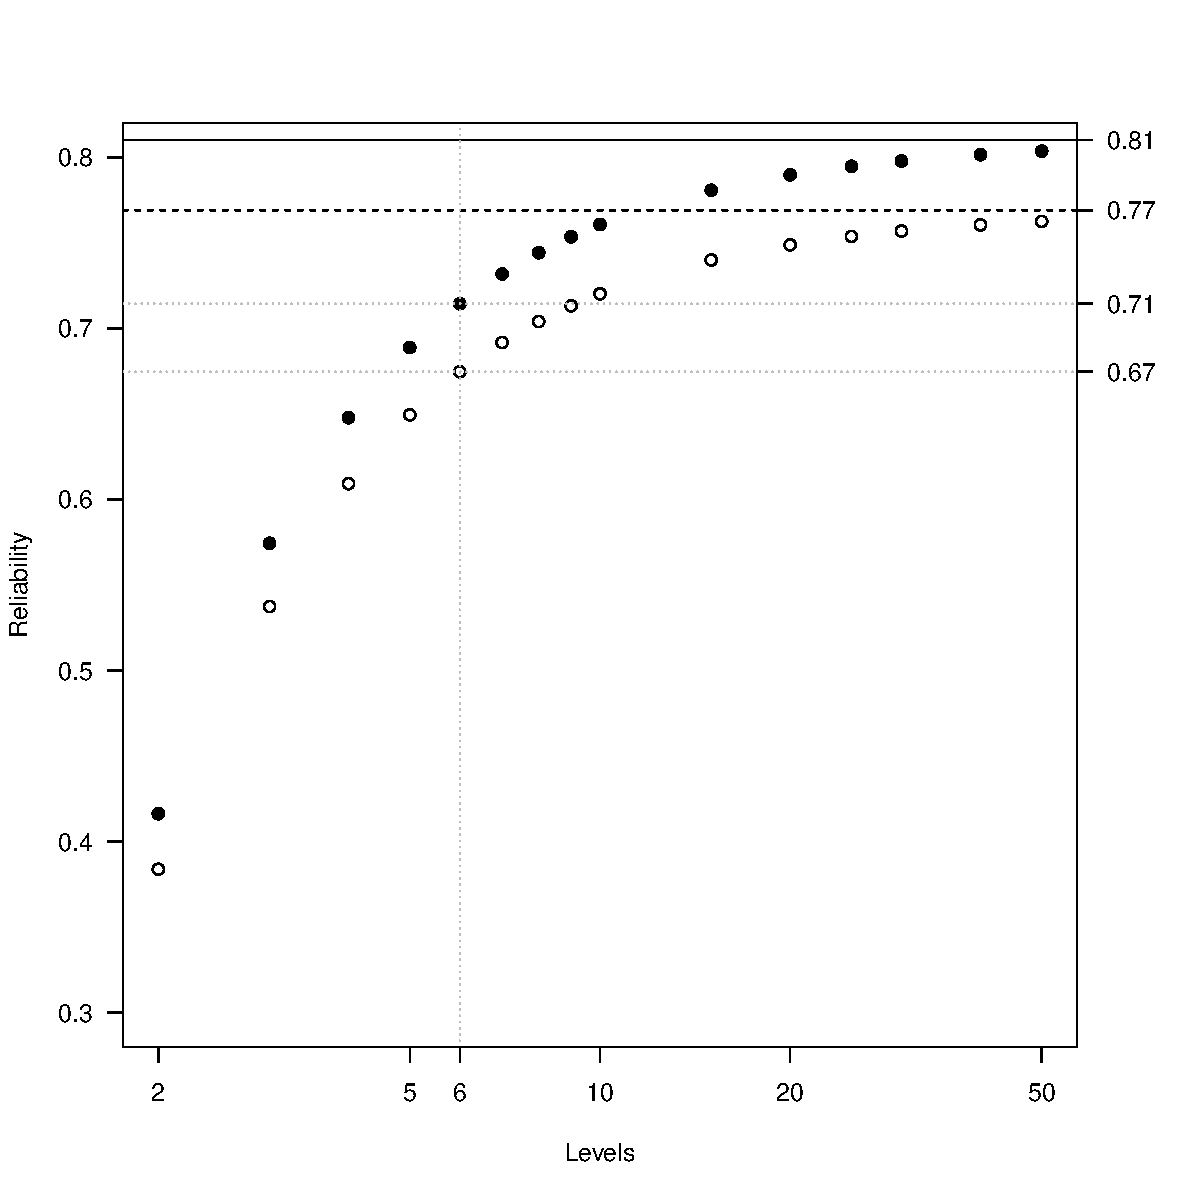
\includegraphics[scale=0.3]{C:/GitHub/standardized/chunks/ordinals}
\par\end{centering}
\caption{\label{fig:Ordinal reliability}Ordinal reliability ($\fullmoon$)
and ordinal $H$ ($\newmoon$) for a selection of Likert levels. The
theoretical coefficient $H$ is $0.81$ (solid line), and the theoretical
composite reliability is $0.77$ (dashed line). All cutoffs are uniform,
and every reliability has been calculated with $\lambda=(0.43,0.71,0.80,0.52,0.67)$
and $\sigma=(0.90,0.70,0.59,0.86,0.74)$. The original number of levels
($6$) and the ordinal reliabilities $(\omega'_{H}=0.71,\omega'=0.67)$
are marked for reference.}
\end{figure}


\section*{Appendix}
\begin{lem}
\label{lem:r^2 and correlation}Assume $Y$ and $\hat{Y}$ have finite
variance. Then 

\begin{equation}
\Cor^{2}(\hat{Y},Y)=1-\frac{\MSE(\alpha+\beta\hat{Y})}{\Var(Y)},\label{eq:rsq and correlation}
\end{equation}
where $\alpha=E(Y)-E(\hat{Y})$ and $\beta=\Cov(\hat{Y},Y)/\Var(\hat{Y})$.
\end{lem}

\begin{proof}
Recenter $Y$ and $\hat{Y}$ so that $E(Y)=E(\hat{Y})=0$. Then 
\begin{eqnarray*}
\MSE(\alpha+\beta\hat{Y}) & = & \beta^{2}\Var(\hat{Y})-2\beta\Cov(\hat{Y},Y)+\Var Y^{2}
\end{eqnarray*}
Differentiate with respect to $\beta$ and set equal to zero, so that
$2\beta\Var(\hat{Y})-2\Cov(\hat{Y},Y)=0$. Then $\beta=\Cov(\hat{Y},Y)/\Var(\hat{Y})$
\end{proof}
%
\begin{proof}[Proof of Theorem (\ref{thm:omega-prime})]
\label{proof:omega-prime}(ii) That $\omega'=1-\MSE(v_{0}\hat{Z})$
follows from Lemma \ref{lem:r^2 and correlation} and the formula
for the covariance, which we now show. The covariance between $\sum_{i=1}^{k}w_{i}\widehat{X}_{i}$
and $Z$ is
\begin{eqnarray*}
\Cov(\sum_{i=1}^{k}w_{i}\widehat{X}_{i},Z) & = & E[\Cov(\sum_{i=1}^{k}w_{i}\widehat{X}_{i},Z\mid\{Y_{i}\})]+\Cov(E\left[\sum_{i=1}^{k}w_{i}\widehat{X}_{i}\mid\{Y_{i}\}\right],E\left[Z\mid\{Y_{i}\}\right]),\\
 & = & -\Cov\left(\sum_{i=1}^{k}w_{i}\widehat{X}_{i},E\left[Z\mid\{Y_{i}\}\right]\right).
\end{eqnarray*}
The expectation $E\left[Z\mid\{Y_{i}=k_{i}\}\right]$ equals $E\left[E\left[Z\mid X\right]\mid\{Y_{i}\}\right]$.
The conditional expectation $E(Z\mid X)=\sum_{i=1}^{k}v_{i}X_{i}$
under multivariate normality, where $v_{i}=\lambda_{i}/[\sigma_{i}^{2}(1+k\overline{\lambda^{2}\sigma^{-2}})]$
are the Thurstone weights, see \citet[Theorem 3.3.4]{Tong1990-lm}.
Consequently, $E[E(Z\mid X)\mid\{Y_{i}\}]=-\sum_{i=1}^{k}v_{i}\hat{X_{i}}$
and 
\begin{eqnarray*}
\Cov(\sum_{i=1}^{k}w_{i}\widehat{X}_{i},Z) & = & \Cov\left(\sum_{i=1}^{k}w_{i}\widehat{X}_{i},\sum_{i=1}^{k}v_{i}\widehat{X}_{i}\right)=w^{T}\Xi v.
\end{eqnarray*}
Standardize to find the correlation $w^{T}\Xi v/\sqrt{w^{T}\Xi w}$,
and the squared correlation is $\omega'=(w^{T}\Xi v)^{2}/w^{T}\Xi w$.
This completes point (i). 

As for (iii), under the parallel model, $v=w_{0}\mathbf{i}$, where
$w_{0}=\lambda/[\sigma^{2}+k\lambda^{2}]$ and the squared correlation
is $w_{0}^{2}\mathbf{i}^{T}\Xi\mathbf{i}=\lambda^{2}\mathbf{i}^{T}\Xi\mathbf{i}/\left(k\lambda^{2}+\sigma^{2}\right)^{2}$.
For the second equation, first notice that
\[
\alpha_{s}=\frac{k}{k-1}\left(\frac{i^{T}\Phi i-k}{i^{T}\Phi i}\right)=k^{2}\left(\frac{\overline{\rho}}{i^{T}\Phi i}\right).
\]
Since $(k\lambda^{2}+\sigma^{2})^{2}=((i^{T}\Phi i)/k)^{2}$, 
\begin{eqnarray*}
\frac{\lambda^{2}}{\left(k\lambda^{2}+\sigma^{2}\right)^{2}}\mathbf{i}^{T}\Xi\mathbf{i} & = & k^{2}\frac{\overline{\rho}}{(i^{T}\Phi i)^{2}}\mathbf{i}^{T}\Xi\mathbf{i},\\
 & = & \alpha_{s}\frac{\mathbf{i}^{T}\Xi\mathbf{i}}{\mathbf{i}^{T}\Psi\mathbf{i}},
\end{eqnarray*}
as claimed.

(i) Follows from the proof (ii); the Thurstone weights optimize $(w^{T}\Xi v)^{2}/w^{T}\Xi w$
since $E[E(Z\mid X)\mid\{Y_{i}\}]=-\sum_{i=1}^{k}v_{i}\hat{X_{i}}$.
\end{proof}
\bibliographystyle{plain}
\bibliography{C:/GitHub/standardized/standardized}

\end{document}
